%programming realization

% \begin{frame}\frametitle{Integration with TVirtualFitter}
\centering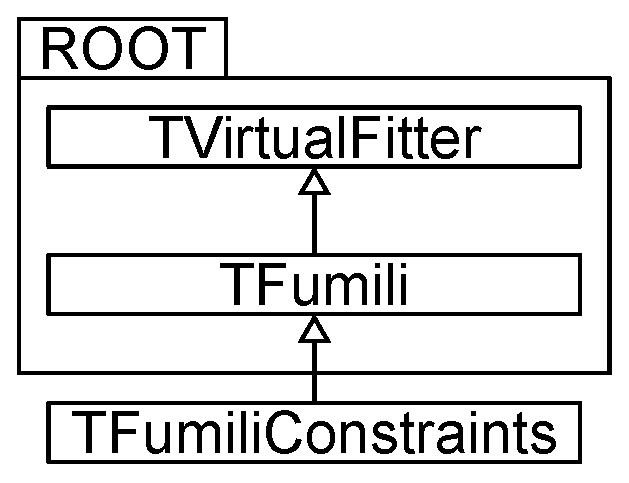
\includegraphics[width=0.7\textwidth]{pics/arch1.eps}
% \end{frame}

% \begin{frame}[fragile]\frametitle{User API}
\footnotesize
% \begin{block}{}
% \begin{lstlisting}
\begin{verbatim}

void FCN(int & n_par, double * grad,
         double & val, double * par, int flag);
/* ... */
TFumiliConstraints * fum = new TFumiliConstraints;
// set parameters
fum->SetParNumber(2);
fum->SetParameter(0, "#alpha", .5, 0.01, 0, 0);
fum->SetParameter(1, "#beta", .0, 0.01, 0, 0);
// set constraints
fum->SetConstrNumber(1);
fum->SetConstraint(0, [](double * p){
  return p[0]*p[0] + .5*p[1] - 1.3;
});
fum->SetConstrDeriv(0, 0, [](double * p){ return 2*p[0]; });
fum->SetConstrDeriv(0, 1, .5);
// set objective function
fum->SetFCN(FCN);
// minimize
fum->Minimize();


\end{verbatim}

% % \end{lstlisting}
% \end{block}
% \end{frame}
